
\begin{frame}{Satellite Foundational Models}
    \centering
    \begin{itemize}
        \item Same performance as ImageNet
    \end{itemize}  
    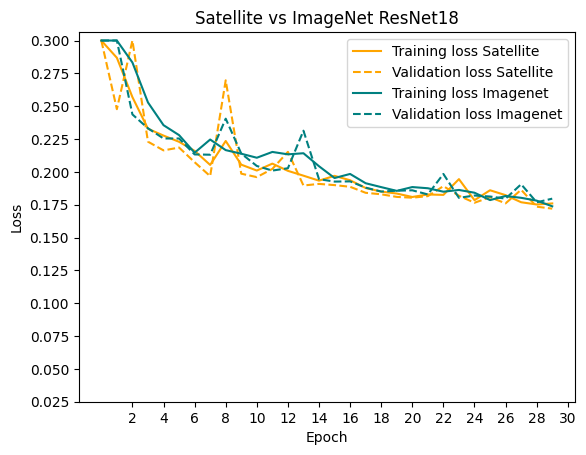
\includegraphics[height=0.6\textheight,width=0.6\textwidth,keepaspectratio]{images/mm_sat_imagenet_loss.png}
    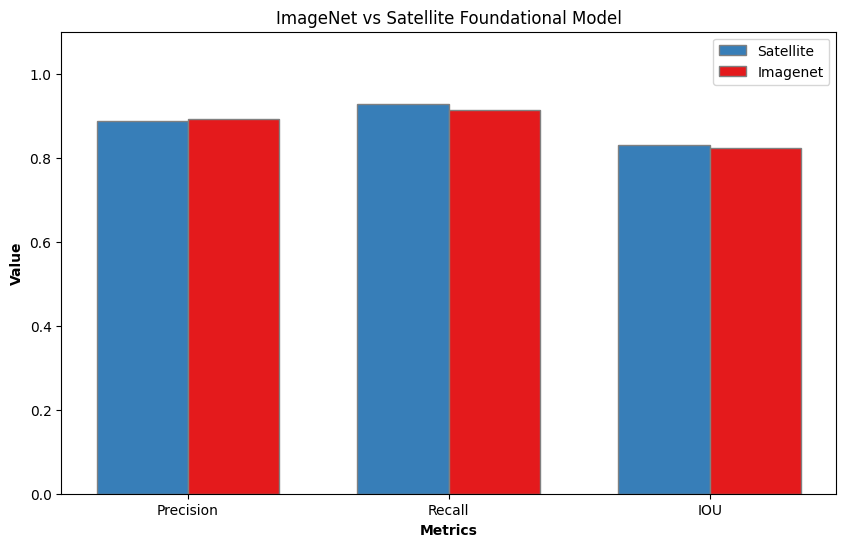
\includegraphics[height=0.6\textheight,width=0.6\textwidth,keepaspectratio]{images/mm_sat_imagenet_performance.png}
\end{frame}

\begin{frame}{BCE vs Jaccard Loss}
    \centering
    \begin{itemize}
        \item Performace improvement with Jaccard Loss
    \end{itemize}  
    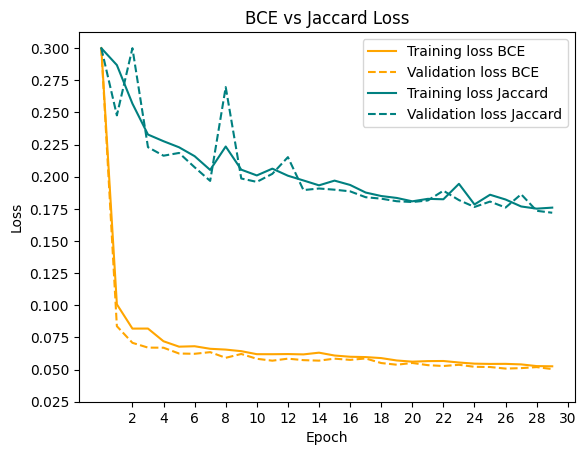
\includegraphics[height=0.6\textheight,width=0.6\textwidth,keepaspectratio]{images/mm_BCE_Jaccard_loss.png}
    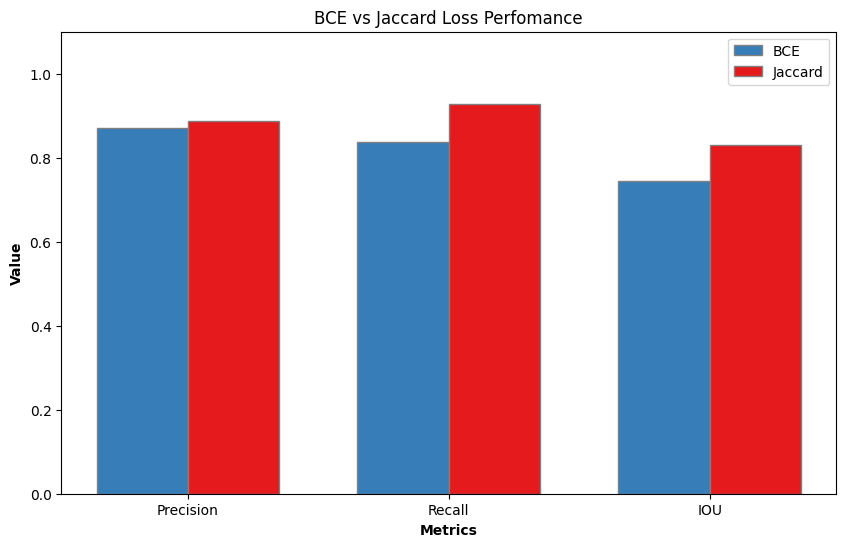
\includegraphics[height=0.6\textheight,width=0.6\textwidth,keepaspectratio]{images/mm_BCE_Jaccard_performance.png}
\end{frame}

\begin{frame}{Old AWS System Architecture}
    \centering
    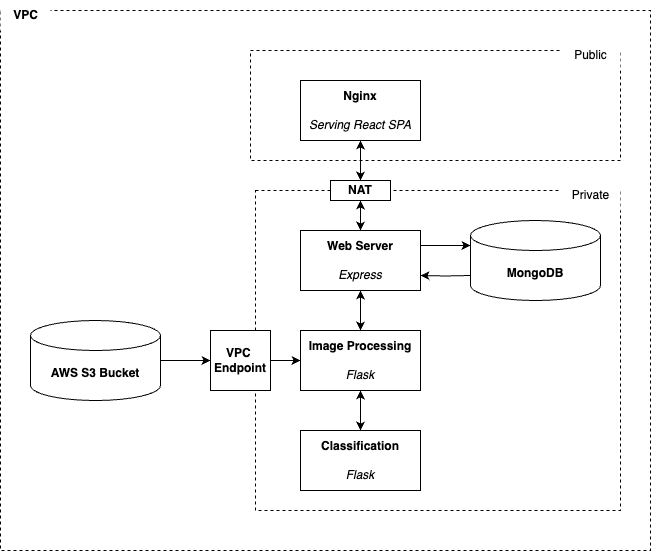
\includegraphics[height=0.8\textheight,width=0.8\textwidth,keepaspectratio]{images/mm_system.png}
\end{frame}

\begin{frame}{AWS Deployment Updates}
    \begin{columns}
        \begin{column}{0.3\textwidth}
            \begin{itemize}
                \item EC2 $\leftrightarrow$ ECS
                \item Exploring networking options
            \end{itemize}  
        \end{column}
        \begin{column}{0.7\textwidth}
            \centering
            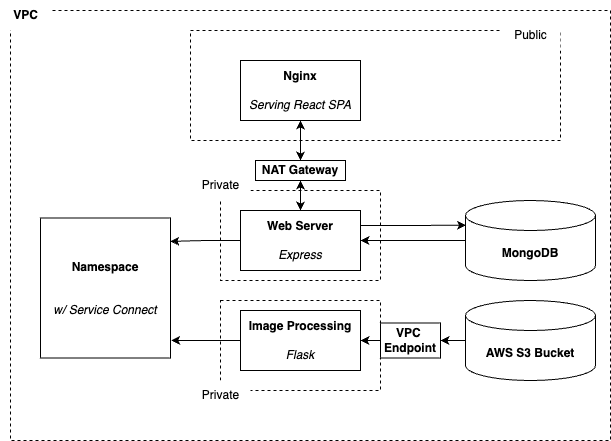
\includegraphics[height=0.8\textheight,width=0.8\textwidth,keepaspectratio]{images/mm_system_2.png}
        \end{column}
    \end{columns}
\end{frame}

\begin{frame}{Image Processing}
    \centering
    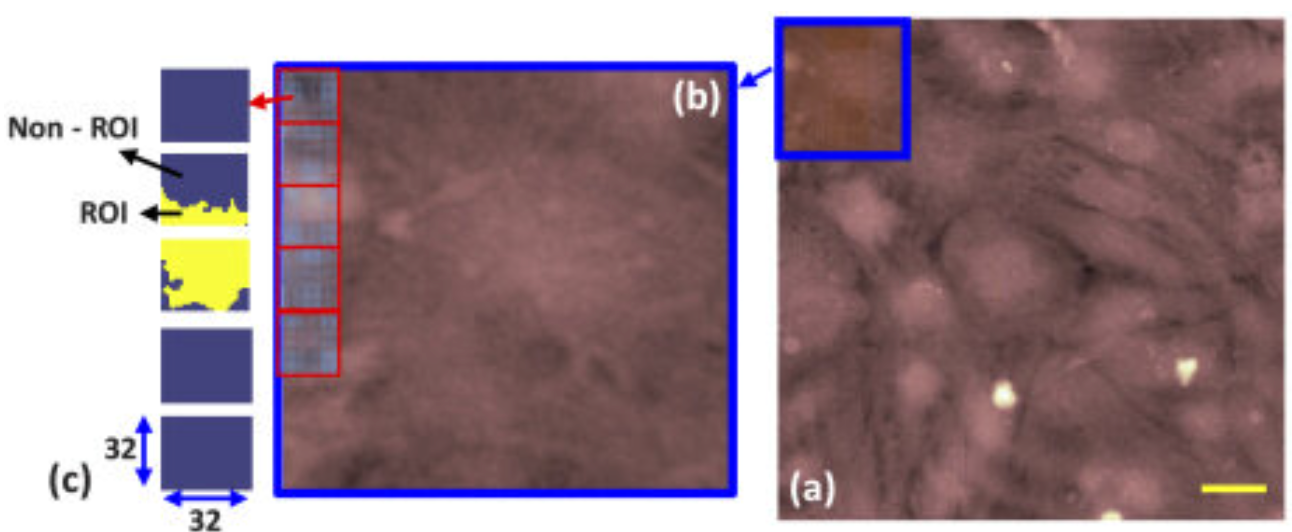
\includegraphics[height=0.7\textheight,width=0.7\textwidth,keepaspectratio]{images/mm_sliding_and_patching.png}
\end{frame}

\begin{frame}{Image Processing}
    \centering
    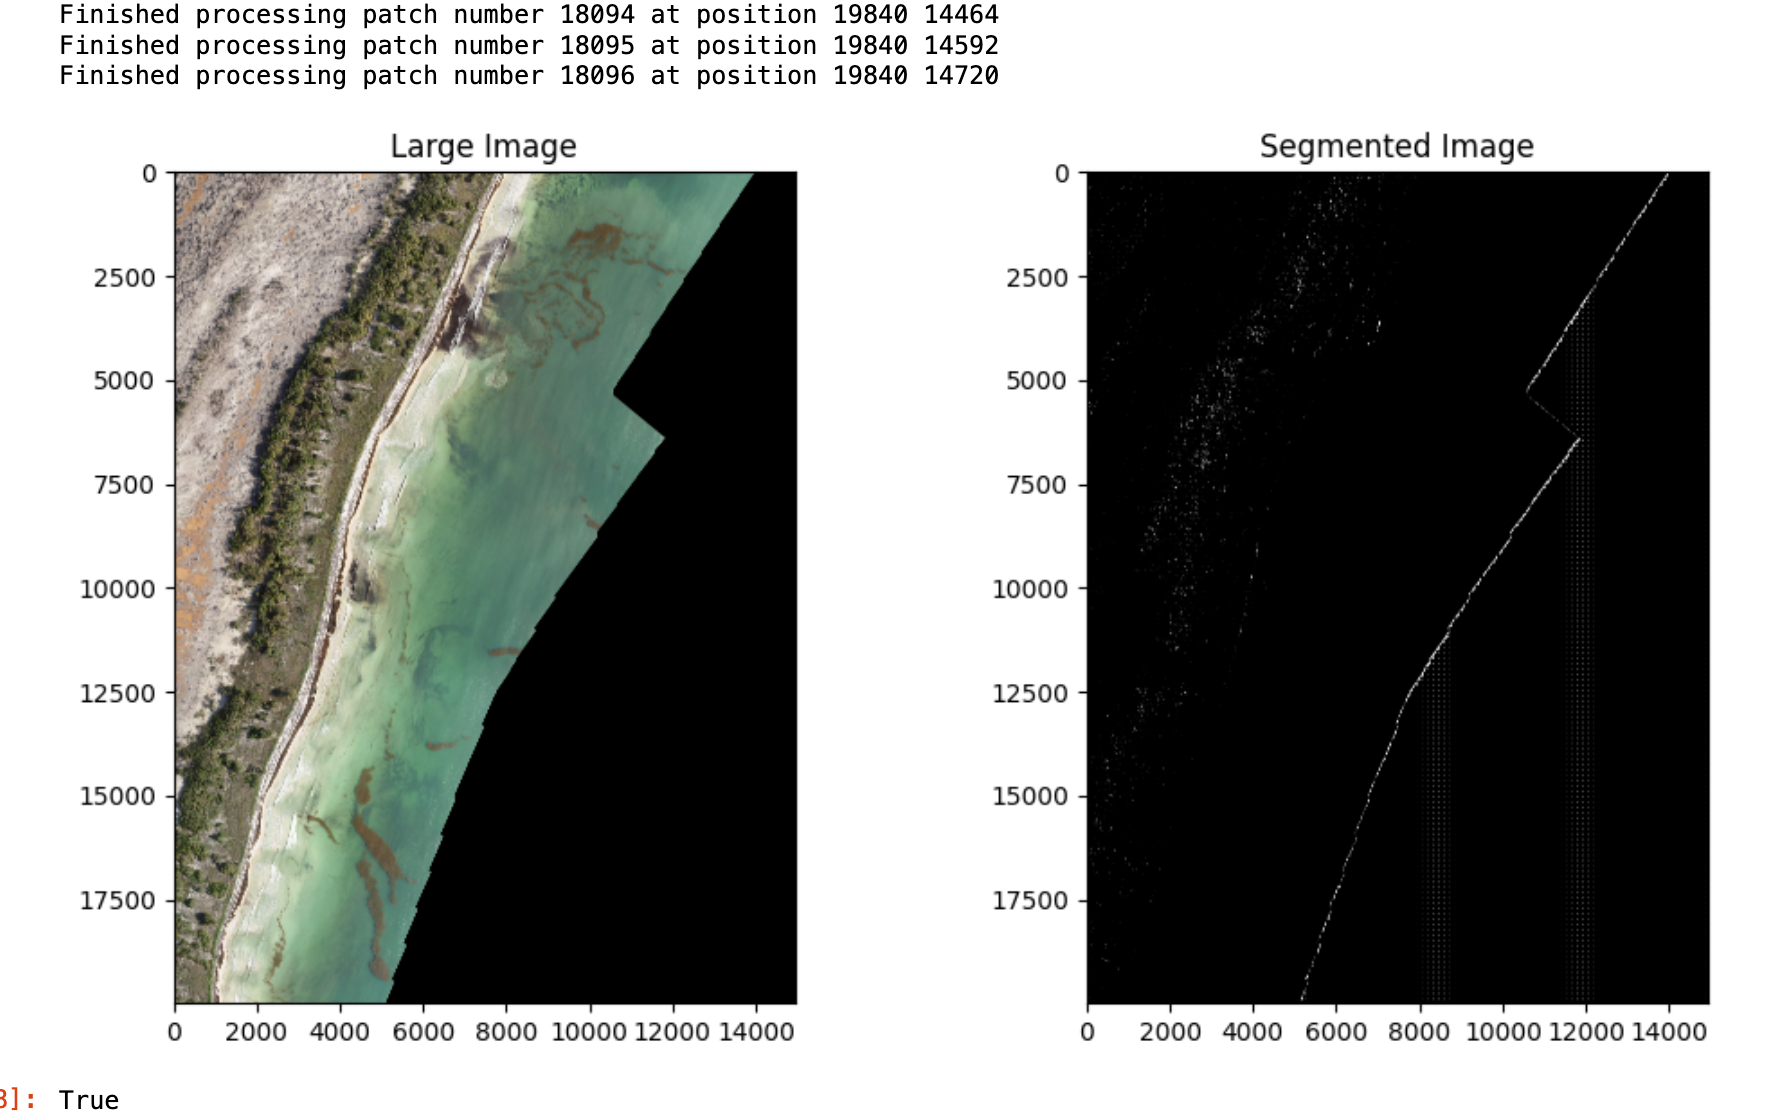
\includegraphics[height=0.7\textheight,width=0.7\textwidth,keepaspectratio]{images/mm_patch.png}
\end{frame}

\begin{frame}{Image Processing}
    \centering
    \begin{minipage}{0.8\textwidth}
        \centering
        \textbf{Using Dummy Pictures} \\[0.5em]
        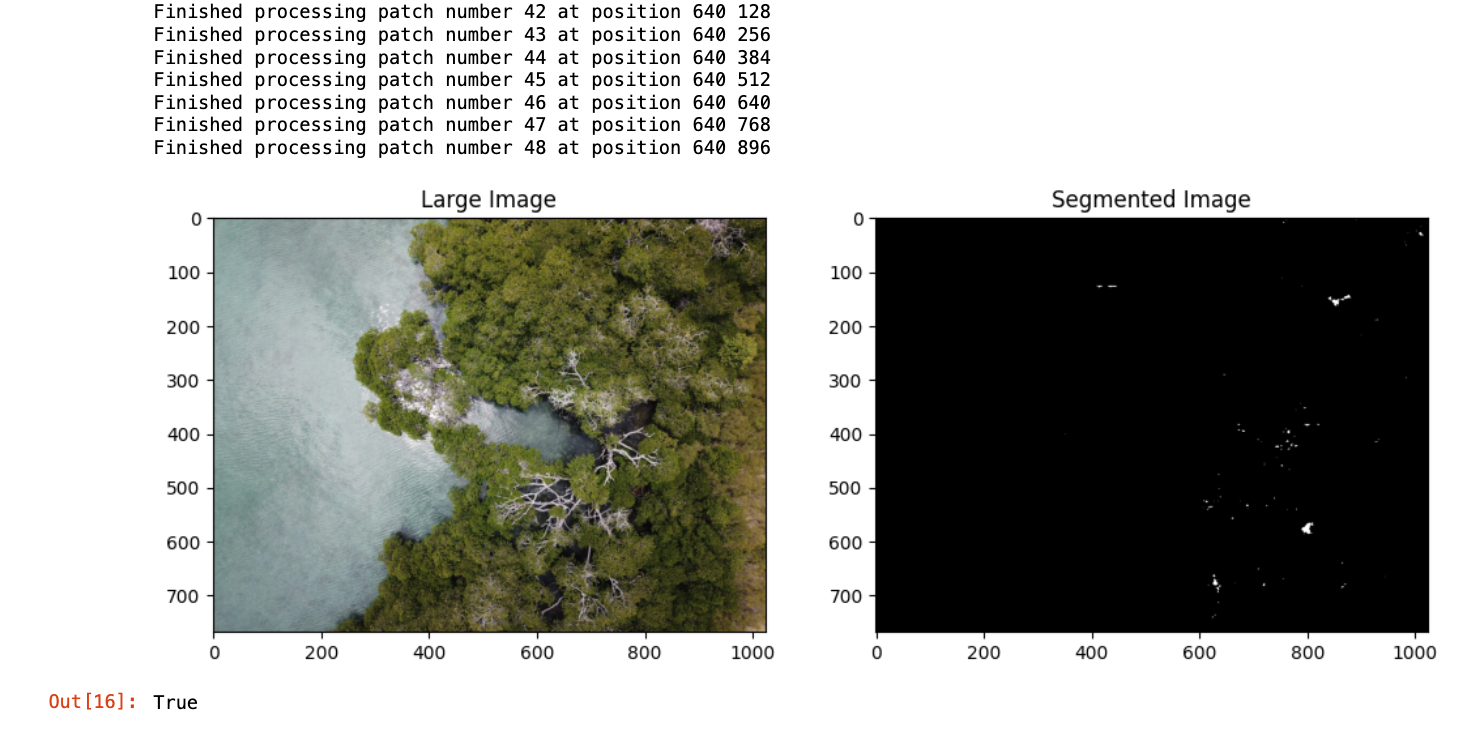
\includegraphics[height=0.35\textheight,width=0.8\textwidth,keepaspectratio]{images/mm_smaller_image.png} \\[1em] % Adjust spacing between images if needed
        \textbf{Downsizing the original picture} \\[0.5em]
        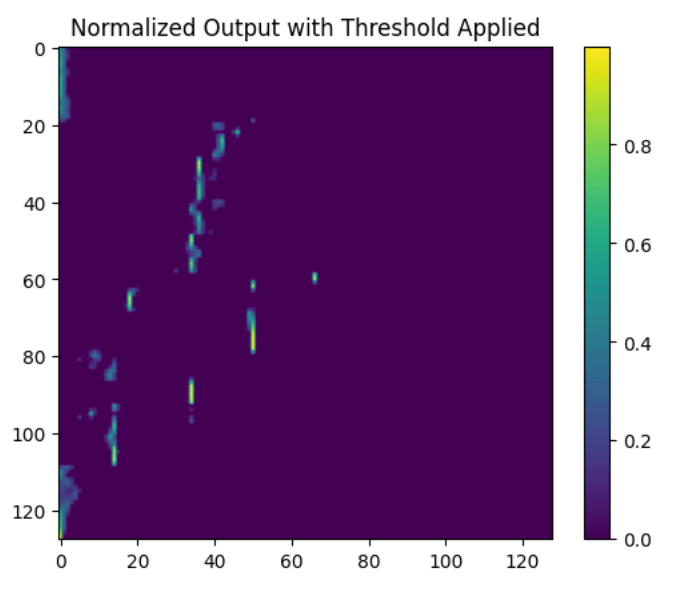
\includegraphics[height=0.35\textheight,width=0.8\textwidth,keepaspectratio]{images/mm_downsizing.png}
    \end{minipage}
\end{frame}




\begin{frame}{Authentication and MongoDB}
    \centering
    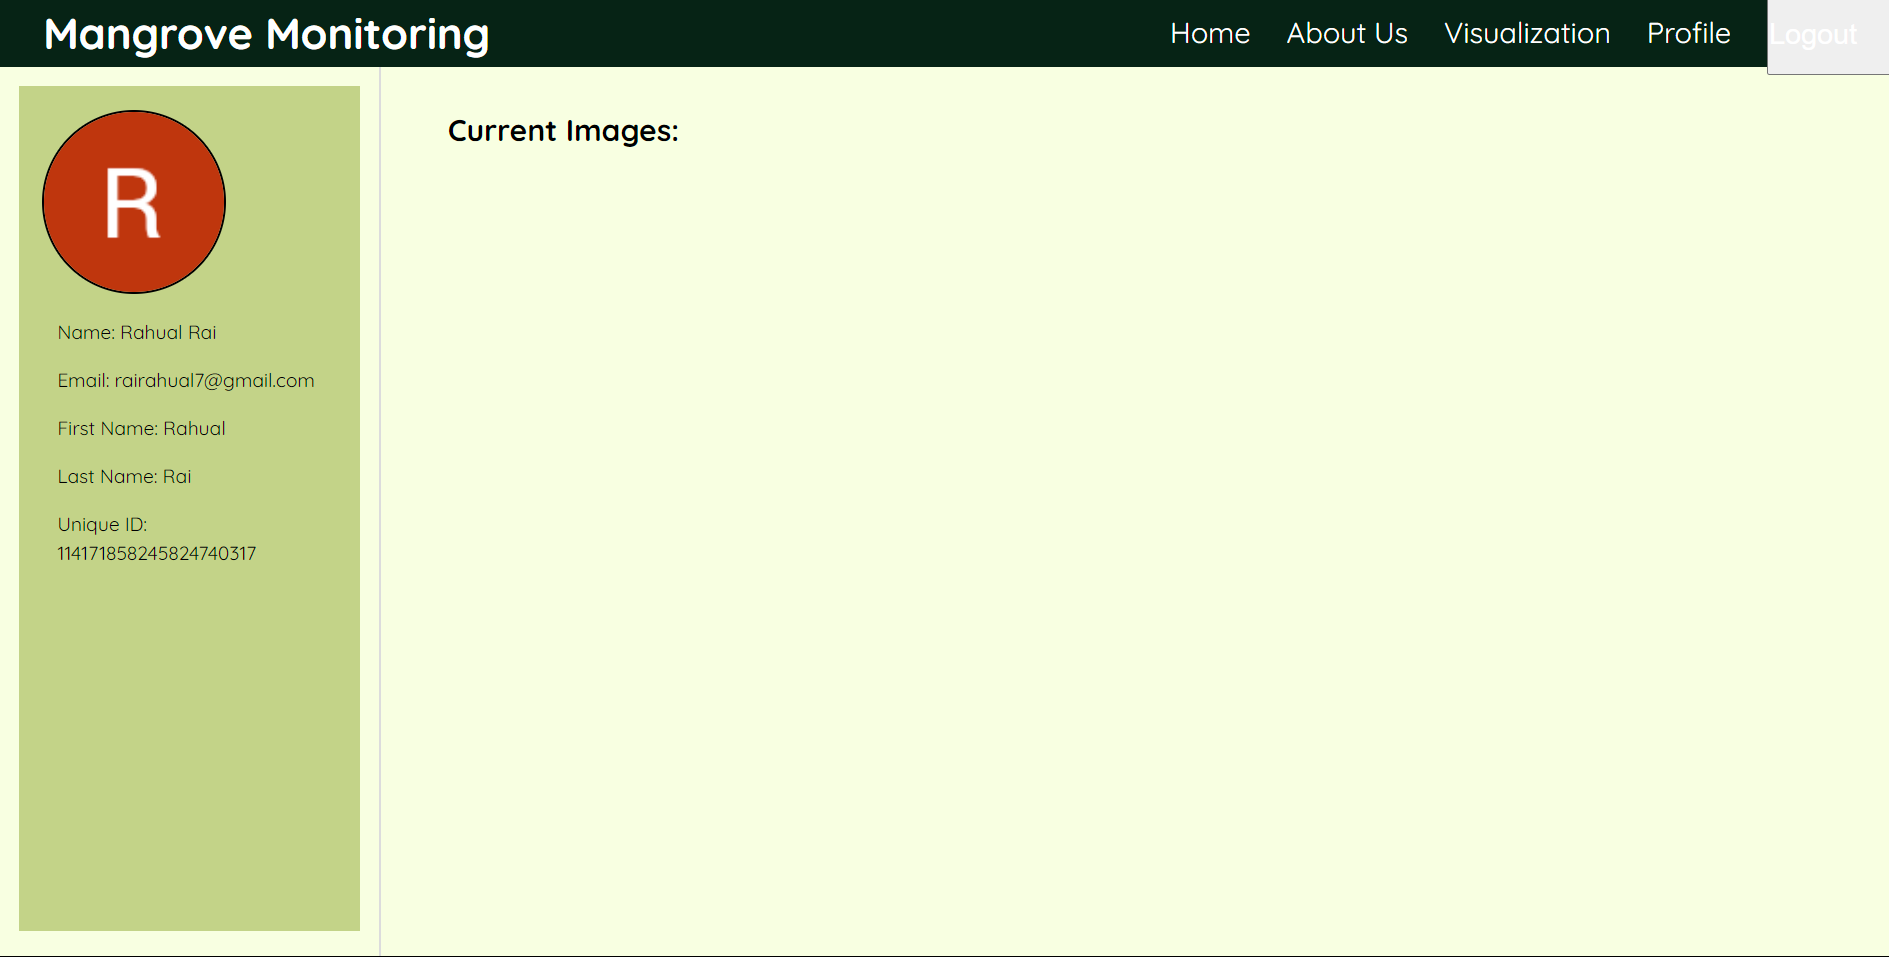
\includegraphics[height=0.7\textheight,width=0.7\textwidth,keepaspectratio]{images/mm_profile.png}
\end{frame}

% To create a slide, use the following:
% \begin{frame}{TITLE}
%     BODY
% \end{frame}

% To create a slide with a bullet list, use the following:
% \begin{frame}{TITLE}
%     \begin{itemize}
%         \item ITEM 1
%         \item ITEM 2
%     \end{itemize}    
% \end{frame}

% To create a slide with numbered list, use the following:
% \begin{frame}{TITLE}
%     \begin{enumerate}
%         \item ITEM 1
%         \item ITEM 2
%     \end{enumerate}
% \end{frame}

% To create a slide with a graphic:
% 1. Add the graphic to this folder (named picture.png)
% 2. Use the following:
% \begin{frame}{TITLE}
%     \centering
%     \includegraphics[height=0.7\textheight,width=0.7\textwidth,keepaspectratio]{picture.png}
% \end{frame}



% To create a slide with two columns, use the following:
% \begin{frame}{TITLE}
%     \begin{columns}
%         \begin{column}{0.5\textwidth}
%             COLUMN 1 BODY
%         \end{column}
%         \begin{column}{0.5\textwidth}
%             COLUMN 2 BODY
%         \end{column}
%     \end{columns}
% \end{frame}
